\section{Two dimensions: further results}\label{supp:two}

\paragraph{The spectra}
The eigendecompositions behind \cref{sec:norm:spectrum} were computed on stiffness matrices
with \numSpecFreeMin{} to \numSpecFreeMax{} free degrees of freedom. When each network's
$\rho$ is first averaged geometrically over its three seeds, which does not pair the seeds
of the two networks, the displacement-supervised transformer's was the larger of the two on
\numSpecLabKnormAboveSeedGm{} of the \numSpecLoadCases{} pairs of instance and load case.
The geometric mean of the ratio of their $\delta^2$ was \numSpecLabKnormDispSeeds{} in seeds
0, 1 and 2, and the displacement-supervised transformer's $\delta$ was the smaller on
\numSpecLabKnormDispLower{} of the triples. The share of the ratio of their relative energy
gaps that the ratio of $\rho$ accounts for, on a logarithmic scale, was
\numSpecSpectralShareMin{} to \numSpecSpectralShareMax{} in the three seeds; in the seed in
which the displacement-supervised transformer's errors were the smaller, the ratio of $\rho$
accounts for more than the whole. This geometric mean is not the ratio of the seed means
that H2a tested, \numCmLabOverKnormGap{}, which the largest errors dominate. The
energy-norm-supervised and the label-free transformers, trained in the same norm, had errors
at the same place in the spectrum (ratio of $\rho$, energy-norm-supervised over label-free,
\numSpecKnormFreeRq{}) and of different sizes (ratio of $\delta^2$ \numSpecKnormFreeDisp{};
\numSpecKnormFreeDispSeeds{} in the three seeds): the energy-norm-supervised transformer's
errors were the smaller in every seed, by far the smaller in seed 1, the seed that makes
most of the difference in H3 (\cref{sec:labelfree:two}). Section~\ref{app:repro:tf32} gives
the readings with TF32 off.

\paragraph{The graph network}
Against the displacement-supervised transformer, instance by instance, the graph network had
the lower displacement error on \numPairCmMgnLabDisp{} of the instance-seed pairs, the lower
relative energy gap on \numPairCmMgnLabGap{} and the lower von Mises error on
\numPairCmMgnLabVm{}.

\paragraph{One instance}
\Cref{fig:field2d} shows one instance, chosen by a rule fixed before the run's spectra were
exported, in the load case that the same rule picks among its four. On that load case, the
four networks' displacement errors lay between \numFigTwoDDispMin{} and \numFigTwoDDispMax{}
and their relative energy gaps between \numFigTwoDGapMin{} and \numFigTwoDGapMax{}; the
stress fields of the two networks trained on the displacement error are visibly rougher.

\begin{figure}[tbp]
\centering
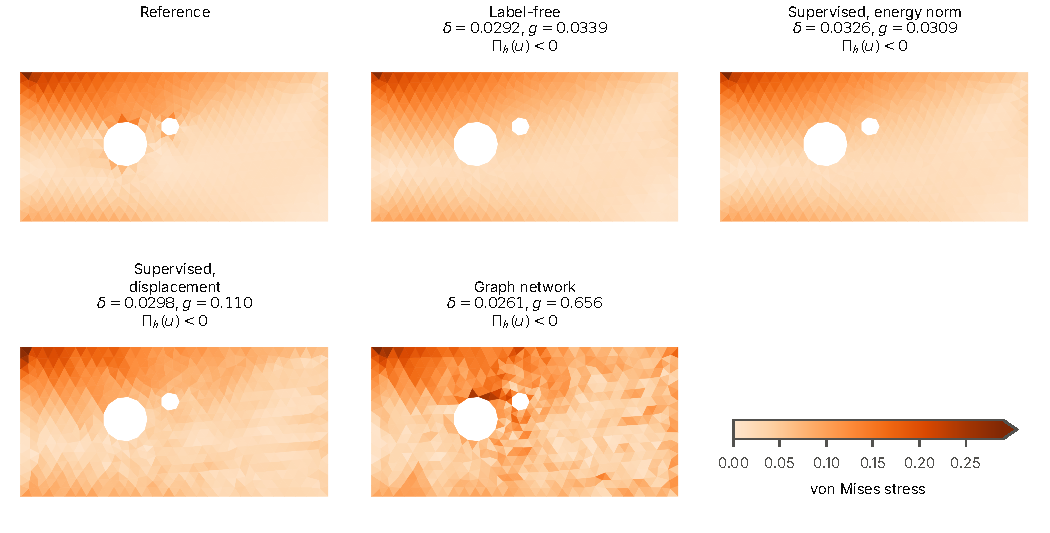
\includegraphics[width=\linewidth]{generated/fig_field2d.pdf}
\caption{Two dimensions, validation instance No.~\numSpecFigIndex{}, the one with the median
relative energy gap of the displacement-supervised transformer, seed 0, under the
\numFigTwoDLoad{} (selection rules in Section~\ref{app:repro:plots}). Von Mises stress of
the reference solution and of the four networks trained on 1,024 instances, on one colour
scale set by the reference. First row: the reference, then the two networks trained in the
energy norm (the label-free and the energy-norm-supervised transformers); second row: the
two trained on the displacement error (the displacement-supervised transformer and the graph
network). Above each network, its relative displacement error $\delta$ and relative energy
gap $g$ on this load case and the sign of $\Pi_h(u)$.}
\label{fig:field2d}
\end{figure}

\paragraph{Fewer labels}
The pre-registration also compared the displacement-supervised and the
energy-norm-supervised transformers with the label-free transformer on every metric at every
number of labels, by the same guard, as readings without verdicts. These are among its
\numCmSecondary{} secondary readings, which are exploratory and not corrected for
multiplicity, so that some crossings of the guard are expected by chance. The
displacement-supervised transformer was worse than the label-free transformer beyond the
guard in relative energy gap, von Mises error, peak stress error and critical-region recall
at every budget. The energy-norm-supervised transformer was worse beyond the guard on every
metric with 16 labelled instances and on every metric but the critical-region recall with
64, and within the guard on every metric with 256 and 1,024; its seed means fell below the
label-free transformer's, in relative energy gap and in displacement, with 1,024 labels
only. Supervised in the energy norm, 256 labelled instances brought the transformer's seed
means within the guard of the label-free transformer's on every metric, although the
label-free transformer still had the lower relative energy gap on
\numPairCmFreeKnormGapTwoFiveSix{} of the instance-seed pairs; supervised on the
displacement error, 1,024 left a von Mises error \numCmLabOverFreeVm{} times the label-free
transformer's.
